\documentclass{llncs}

\usepackage{textcomp}
\usepackage{listings}
\usepackage{pgfplots}
\usepackage{SIunits} 
\usepackage[utf8]{inputenc}
\usepackage{subcaption}
\captionsetup{compatibility=false}
\usepackage{float}
\usepackage{chngcntr}
\usepackage{placeins}
\usepackage[british]{babel}
\usepackage{xcolor}
\PassOptionsToPackage{hyphens}{url}\usepackage{hyperref}
\setcounter{tocdepth}{3}
\pgfplotsset{compat=newest}

\definecolor{mGreen}{rgb}{0,0.6,0}
\definecolor{mGray}{rgb}{0.5,0.5,0.5}
\definecolor{mPurple}{rgb}{0.58,0,0.82}
\definecolor{backgroundColour}{rgb}{0.95,0.95,0.92}

\lstdefinestyle{CStyle}{
    backgroundcolor=\color{backgroundColour},   
    commentstyle=\color{mGreen},
    keywordstyle=\color{magenta},
    numberstyle=\tiny\color{mGray},
    stringstyle=\color{mPurple},
    basicstyle=\footnotesize,
    breakatwhitespace=false,         
    breaklines=true,                 
    captionpos=b,                    
    keepspaces=true,                 
    numbers=left,                    
    numbersep=5pt,                  
    showspaces=false,                
    showstringspaces=false,
    showtabs=false,                  
    tabsize=2,
    language=C
}
\lstdefinestyle{JavaStyle}{
    backgroundcolor=\color{backgroundColour},   
    commentstyle=\color{mGreen},
    keywordstyle=\color{magenta},
    numberstyle=\tiny\color{mGray},
    stringstyle=\color{mPurple},
    basicstyle=\footnotesize,
    breakatwhitespace=false,         
    breaklines=true,                 
    captionpos=b,                    
    keepspaces=true,                 
    numbers=left,                    
    numbersep=5pt,                  
    showspaces=false,                
    showstringspaces=false,
    showtabs=false,                  
    tabsize=2,
    language=Java
}



\graphicspath{ {Graphs/} }




\begin{document}


\title{Linear Correlation on Maxeler}

\author{Christian Permann}

\institute{Faculty of Computer Science, University of Vienna,\newline W\"ahringer Stra{\ss}e 29, 1090 Vienna}
\maketitle

\begin{abstract}
This paper explains the very basics of Linear Correlation (Pearson Correlation) and how to trivialy implement it on a Maxeler architecture. This should result in a high speedup, since the calculations can benefit a lot from the DataFlow paradigm.
\end{abstract}

\tableofcontents
%\clearpage

\section{Introduction}\label{sec:into}
Linear Correlation is an important analysis method to find how well two variables correlate with each other. Thereby the value of r is to be considered, which is defined by:

$$r = \frac{\Sigma(x_i - \bar{x})(y_i - \bar{y})}{\sqrt{\Sigma(x_i - \bar{x})^2\Sigma(y_i - \bar{y})^2}}$$
\newline

This variable r(Pearson Correlation Coefficient) can take on values in the interval \(\left[-1, +1\right]\), whereas -1 indicates perfect indirect linear correlation, 0 indicates no linear correlation and +1 indicates perfect direct linear correlation. The emphasis lies on \emph{linear} correlation because there still may be higher order or non-trivial correlations, like cyclic ones. This is an important consideration because a low absolute correlation value here does not suffice as proof that the analysed variables are generaly independent. 

Here the Pearson Correlation is used, but there also exist other Linear Correlation variants like Rank Correlation (Spearman's Correlation). The main difference of this method is, that the size of the variables actually matters and not only their ranking relative to each other. This can be dependent on the problem to be analysed be an advantage or disadvantage in comparison to Rank Correlation.

Such a calculation may be especialy interesting in fields like statistical analysis, where it is a common method for a quick first analysis. Here it is often used with many variables and correlating them all against eachother, which may result in lots of computation runs. Finding a high absolute value for the correlation coefficient here may allow to disregard some of the variables in further analysis since they can be derived linearly form other variables. This should usualy just be done though, if the following methods of analysis do also take linear relationships into regard.

\section{Classical Implementation}\label{sec:Classical_Implementation}

The usual implementation of the calculation of the Pearson Correlation Coefficient, as seen in Listing \ref{lst:CImplementation}, spends most of its time within loops.

\begin{lstlisting}[style=CStyle,label={lst:CImplementation},caption={Implementation in C, modified from \cite{Press:1988:NRC:42249}},captionpos=b]
#define TINY 1.0e-20

unsigned long j;
float yt,xt,r;
float syy=0.0,sxy=0.0,sxx=0.0,ay=0.0,ax=0.0;
for (j=1;j<=n;j++) { //Find the means.
	ax += x[j];
	ay += y[j];
}
ax /= n;
ay /= n;
for (j=1;j<=n;j++) { //Compute the correlation coefficient.
	xt=x[j]-ax;
	yt=y[j]-ay;
	sxx += xt*xt;
	syy += yt*yt;
	sxy += xt*yt;
}
r=sxy/(sqrt(sxx*syy)+TINY); 
\end{lstlisting}

The time spent in those loops is the reason why this algorithm can be run on the maxeler architecture efficiently. While the usual ControlFlow paradigm has to load the data objects and instructions sequencially (even though this may be reduced by vectorizing), those instructions can be executed on a DataFlow machine by just steaming in data.

\section{Maxeler Implementation}\label{sec:Maxeler_Implementation}

The trivial case of calculating the Pearson Correlation Coefficient for arrays of fixed length is implemented very simmilarly to C or normal Java, the only real difference is that one has to be careful when choosing between classical Java variables and Maxeler defined variables.

\begin{lstlisting}[style=JavaStyle,label={lst:JavaImplementation},caption={Implementation in Maxeler Java},captionpos=b]
DFEVar n=constant.var(dfeFloat(8, 24), vectorSize);
DFEVar ax=constant.var(dfeFloat(8, 24), 0);
DFEVar ay=constant.var(dfeFloat(8, 24), 0);
DFEVectorType<DFEVar> vectorType = new DFEVectorType<DFEVar>(dfeFloat(8,24), vectorSize);

DFEVector<DFEVar> inVector = io.input("inVector", vectorType);
DFEVector<DFEVar> inVector2 = io.input("inVector2", vectorType);
for (int i = 0; i < vectorSize; i++){
	ax+=inVector[i];
	ay+=inVector2[i];
}
ax/=n;
ay/=n;

DFEVar xt=constant.var(dfeFloat(8, 24), 0);
DFEVar yt=constant.var(dfeFloat(8, 24), 0);
DFEVar sxx=constant.var(dfeFloat(8, 24), 0);
DFEVar syy=constant.var(dfeFloat(8, 24), 0);
DFEVar sxy=constant.var(dfeFloat(8, 24), 0);
for (int i = 0; i < vectorSize; i++){
	xt = inVector[i]-ax;
	yt = inVector2[i]-ay;
	sxx += xt*xt;
	syy += yt*yt;
	sxy += xt*yt;
}
DFEVar r = sxy/(KernelMath.sqrt(sxx*syy)+1.0e-20);

io.output("outScalar", r, dfeFloat (8, 24));
\end{lstlisting}

With this simple piece of code, the maxeler compiler is able to build a DataFlow graph and rewire an FPGA to execute the code. Doing this allows to trade space on the FPGA for more performance or in this case larger problem sizes, while achieving a high speedup. Another advantage could be that the numeric precision can be increased arbitrarily while not loosing as much performance (space) as if using arbitrary precision libraries on a classical ControlFlow machine. 

\subsection{Maxeler Execution Graph}\label{sec:Maxeler_Execution_Graph}

As already mentioned, an execution graph is generated by the Maxeler compiler which visualizes how the FPGA will be reprogrammed. The execution graph for this example can be seen in Figure \ref{fig:execution_graph}.

\begin{figure}
\begin{center}
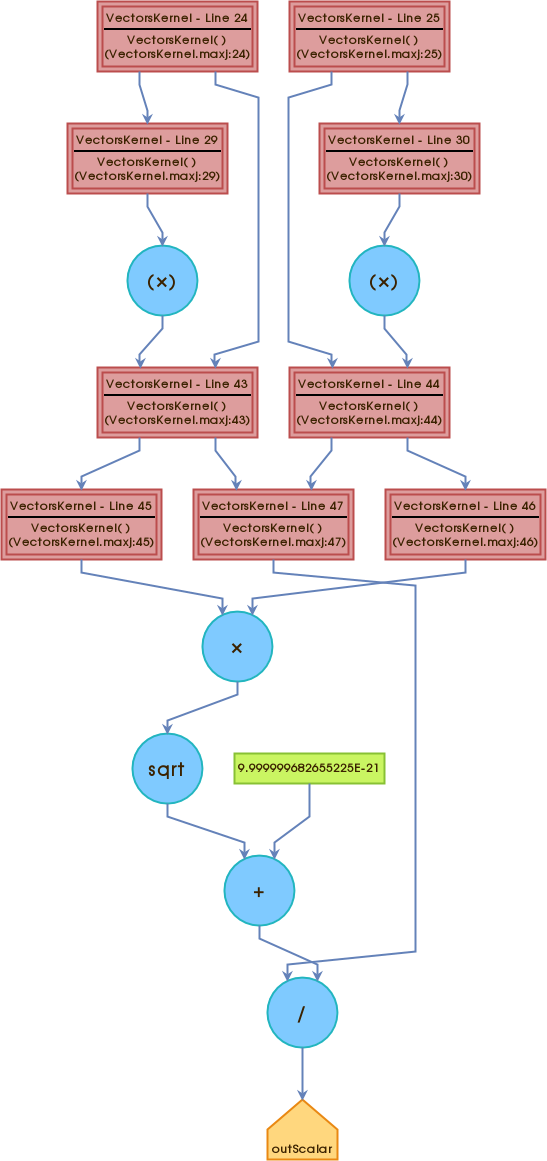
\includegraphics[width=0.7\textwidth]{Vectors-VectorsKernel-final-simulation}
\end{center}
\caption{Execution graph for calculating r}
\label{fig:execution_graph}
\end{figure}


\section{Conclusion}\label{sec:Conclusion}

The implementation of the calculation of the Pearson Correlation Coefficient shows nicely what Maxeler can be used for. This is a trivial first example that shows especialy well how IO works and the different variable types. The proposed solution and code written in Maxeler Java could still be improved to for example allow for varying array sizes durring runtime, aswell as returning intermediate results. Depending on the application this may not be needed though, omiting these features can save on space on the FPGA and may therefor allow for calculating larger problem sizes.

\section*{Acknowledgments}\label{sec:Acknowledgments}

The author would like to thank Milos Kotlar and Prof. Veljko M. Milutinovic for their teachings on the subject of Maxeler and DataFlow computing.

\bibliographystyle{splncs03}

\bibliography{citations}

\end{document}
